\documentclass[11pt,a4paper]{article}

\usepackage[margin=1in]{geometry}
\usepackage{graphicx}
\usepackage[font=small,labelfont=bf]{caption}
\usepackage{hyperref}
\usepackage{enumitem}
\usepackage{booktabs}
\usepackage{amsmath,amssymb}
\usepackage{xcolor}
\usepackage{fancyhdr}
\usepackage{titlesec}
\usepackage{listings}
\usepackage{tabularx}

\graphicspath{{images/}{./images/}}
\newcommand{\imgwidth}{0.92\textwidth}

\definecolor{navy}{HTML}{1B2A4A}
\definecolor{linkblue}{HTML}{2B6CB0}

\hypersetup{
    colorlinks=true,
    linkcolor=navy,
    urlcolor=linkblue,
    citecolor=navy,
}

\titleformat{\section}{\Large\bfseries\color{navy}}{\thesection}{1em}{}
\titleformat{\subsection}{\large\bfseries\color{navy!80}}{\thesubsection}{1em}{}
\titleformat{\subsubsection}{\normalsize\bfseries\color{navy!60}}{\thesubsubsection}{1em}{}

\pagestyle{fancy}
\fancyhf{}
\fancyhead[L]{\small\textcolor{gray}{GSoC 2026 Proposal}}
\fancyhead[R]{\small\textcolor{gray}{Healing Stone: Automated Fragment Reconstruction}}
\fancyfoot[C]{\thepage}
\renewcommand{\headrulewidth}{0.4pt}

\lstset{
    basicstyle=\ttfamily\small,
    backgroundcolor=\color{gray!5},
    frame=single,
    rulecolor=\color{gray!30},
    breaklines=true,
    columns=fullflexible,
}

\title{
    \vspace{-1cm}
    {\Huge\textbf{\textcolor{navy}{Healing Stone}}} \\[0.3cm]
    {\Large Automated Reconstruction of Fragmented Cultural Artifacts} \\[0.3cm]
    {\large Google Summer of Code 2026 Proposal}
}
\author{
    Ujjwal Singh \\
    \href{mailto:ujjosing@gmail.com}{ujjosing@gmail.com} \\
    \url{https://github.com/fallofpheonix}
}
\date{}

\begin{document}
\maketitle
\thispagestyle{fancy}

\vspace{-0.5cm}
\begin{center}
\rule{0.8\textwidth}{0.5pt}
\end{center}

%==============================================================================
\tableofcontents
\newpage

%==============================================================================
\section{Abstract}

Fragmented cultural artifacts present one of the most challenging problems in computational archaeology. Erosion, incomplete scans, and noisy geometry render manual reconstruction infeasible at scale. This proposal presents \textbf{Healing Stone}, a hybrid geometric and learning-based pipeline that automates the full lifecycle of fragment reconstruction: preprocessing, feature extraction, pairwise matching, rigid alignment, validation, and global assembly.

The system is engineered with three non-negotiable invariants: \textbf{hard determinism} (100\% reproducibility across environments), \textbf{typed data contracts} (Pydantic-validated configurations and metrics), and \textbf{formal evaluation} (quantitative benchmarks against established baselines). The pipeline supports both 3D mesh fragments (\texttt{.ply/.obj}) and 2D image fragments (\texttt{.png/.jpg}), with automatic input detection.

The proposed GSoC work extends the existing prototype into a production-grade system by hardening validation gates, introducing adversarial robustness testing, expanding the evaluation suite, and documenting the system to research-publication standards.

%==============================================================================
\section{Problem Statement}

\subsection{The Archaeological Challenge}

Cultural heritage preservation demands the reconstruction of artifacts fragmented by natural erosion, excavation damage, or historical destruction. Current workflows rely on domain experts manually fitting fragments — a process that does not scale beyond dozens of pieces and is inherently subjective.

\subsection{Technical Gaps in Existing Approaches}

\begin{enumerate}[leftmargin=*]
    \item \textbf{Geometric-only methods} (e.g., ICP-based registration) fail under surface erosion, where contact surfaces lose distinctive features.
    \item \textbf{Purely learned systems} (e.g., end-to-end neural reassembly) lack interpretability and produce no traceable validation artifacts.
    \item \textbf{Ad-hoc pipelines} lack determinism, structured data transformations, and formal evaluation — making results non-reproducible.
\end{enumerate}

\subsection{Current Baseline}

As shown in Figure~\ref{fig:pipeline}, the existing pipeline implements a linear stage-based flow with explicit decision points. However, the validation gates require hardening, the evaluation suite needs expansion, and the documentation requires formalization for research dissemination.

\begin{figure}[htbp]
    \centering
    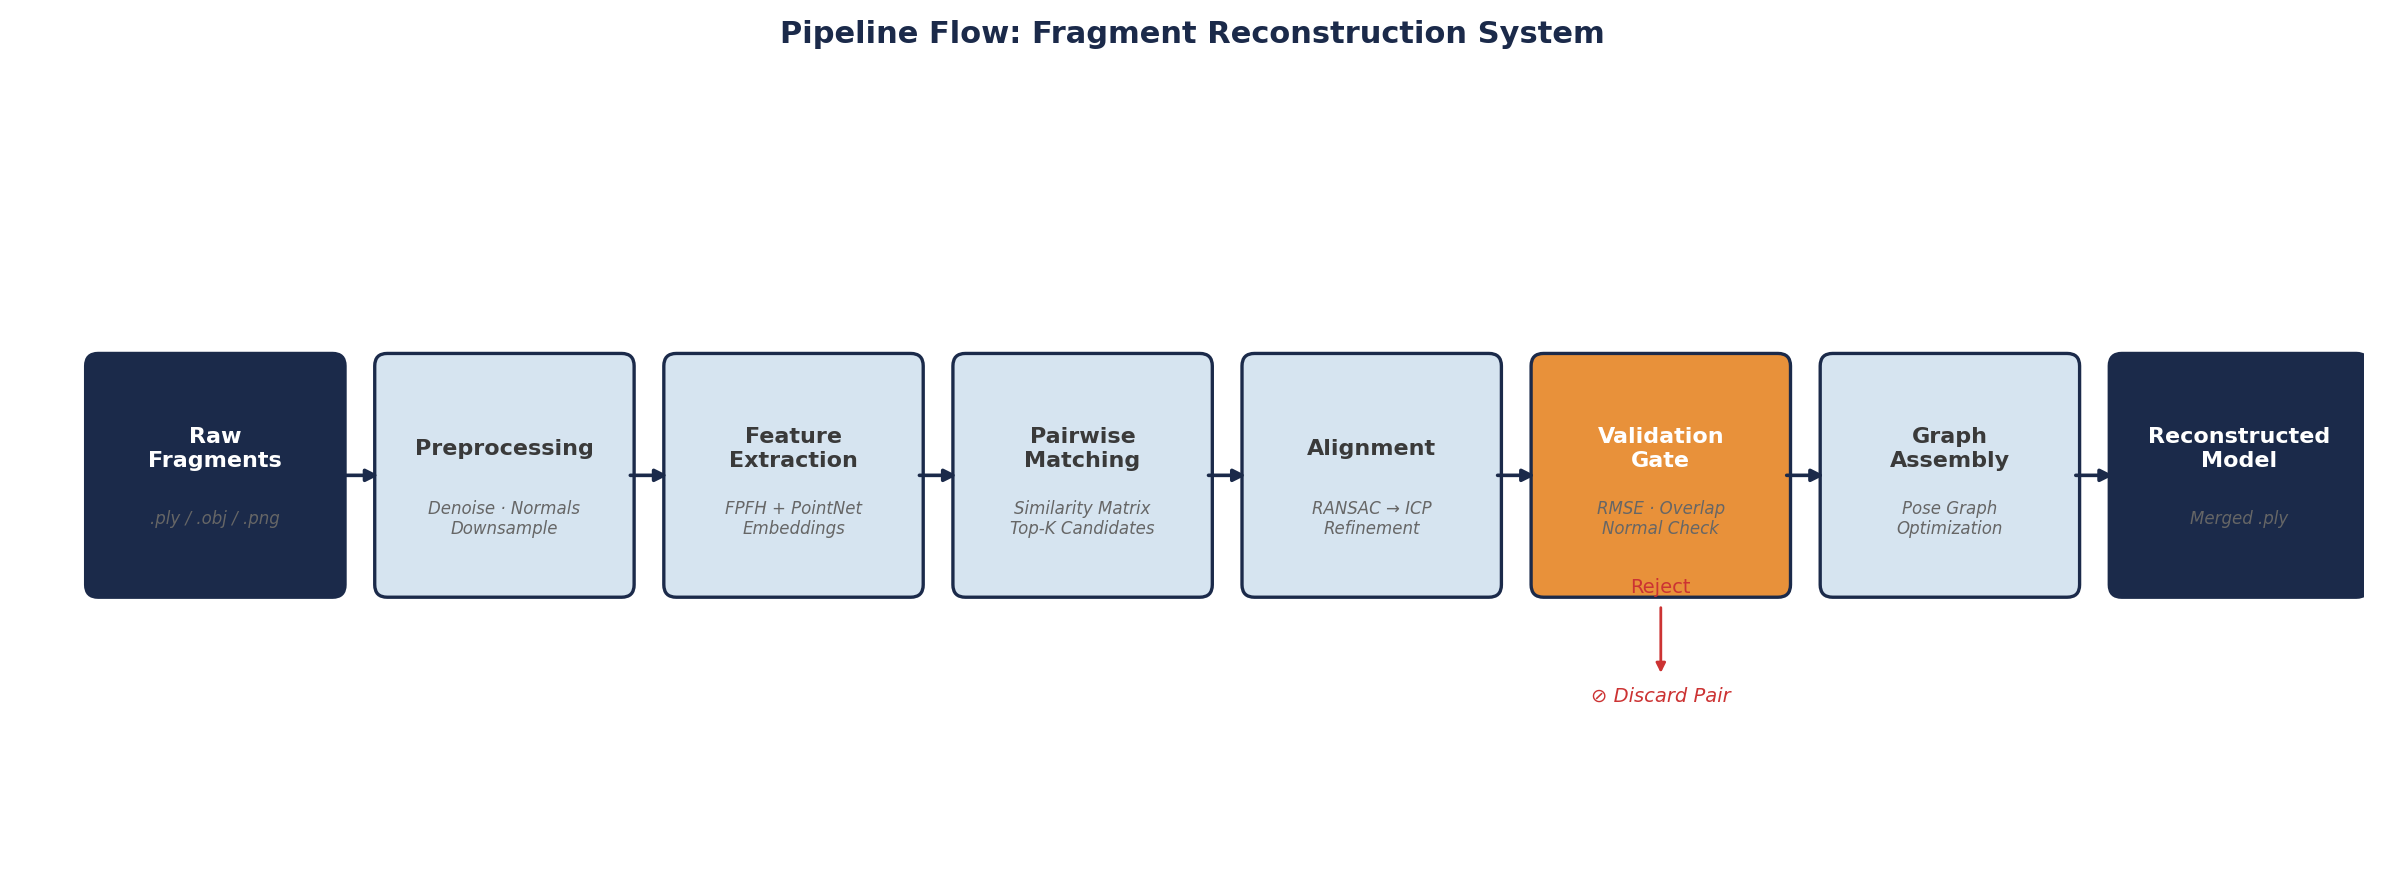
\includegraphics[width=\imgwidth]{pipeline.png}
    \caption{End-to-end pipeline flow with validation gate and reject path. Each stage produces typed intermediate artifacts enabling traceability and debugging.}
    \label{fig:pipeline}
\end{figure}

%==============================================================================
\section{Proposed Solution}

The proposed system is a \textbf{modular, deterministic pipeline} that combines geometric descriptors (FPFH) and learned embeddings (PointNet) for matching, coarse-to-fine alignment (RANSAC $\rightarrow$ ICP) with validation, and graph-based assembly with conflict resolution.

\subsection{Key Design Principles}

\begin{itemize}[leftmargin=*]
    \item \textbf{Hybrid Feature Representation}: Geometric FPFH descriptors provide domain-specific surface information, while learned PointNet embeddings capture higher-order structural relationships.
    \item \textbf{Explicit Validation Gates}: Every alignment is validated against RMSE thresholds, overlap ratios, and normal consistency before entering the assembly graph.
    \item \textbf{Deterministic Execution}: Centralized seed management across NumPy, PyTorch, and CUDA ensures bitwise-identical results across runs.
    \item \textbf{Typed Artifacts}: Every intermediate output conforms to a Pydantic schema, enabling automated validation and downstream consumption.
\end{itemize}

%==============================================================================
\section{System Architecture}

\subsection{Layered Design}

The system follows a strict layered architecture (Figure~\ref{fig:architecture}) where each layer exposes typed interfaces to adjacent layers. This design prevents circular dependencies and enables independent testing of each component.

\begin{figure}[htbp]
    \centering
    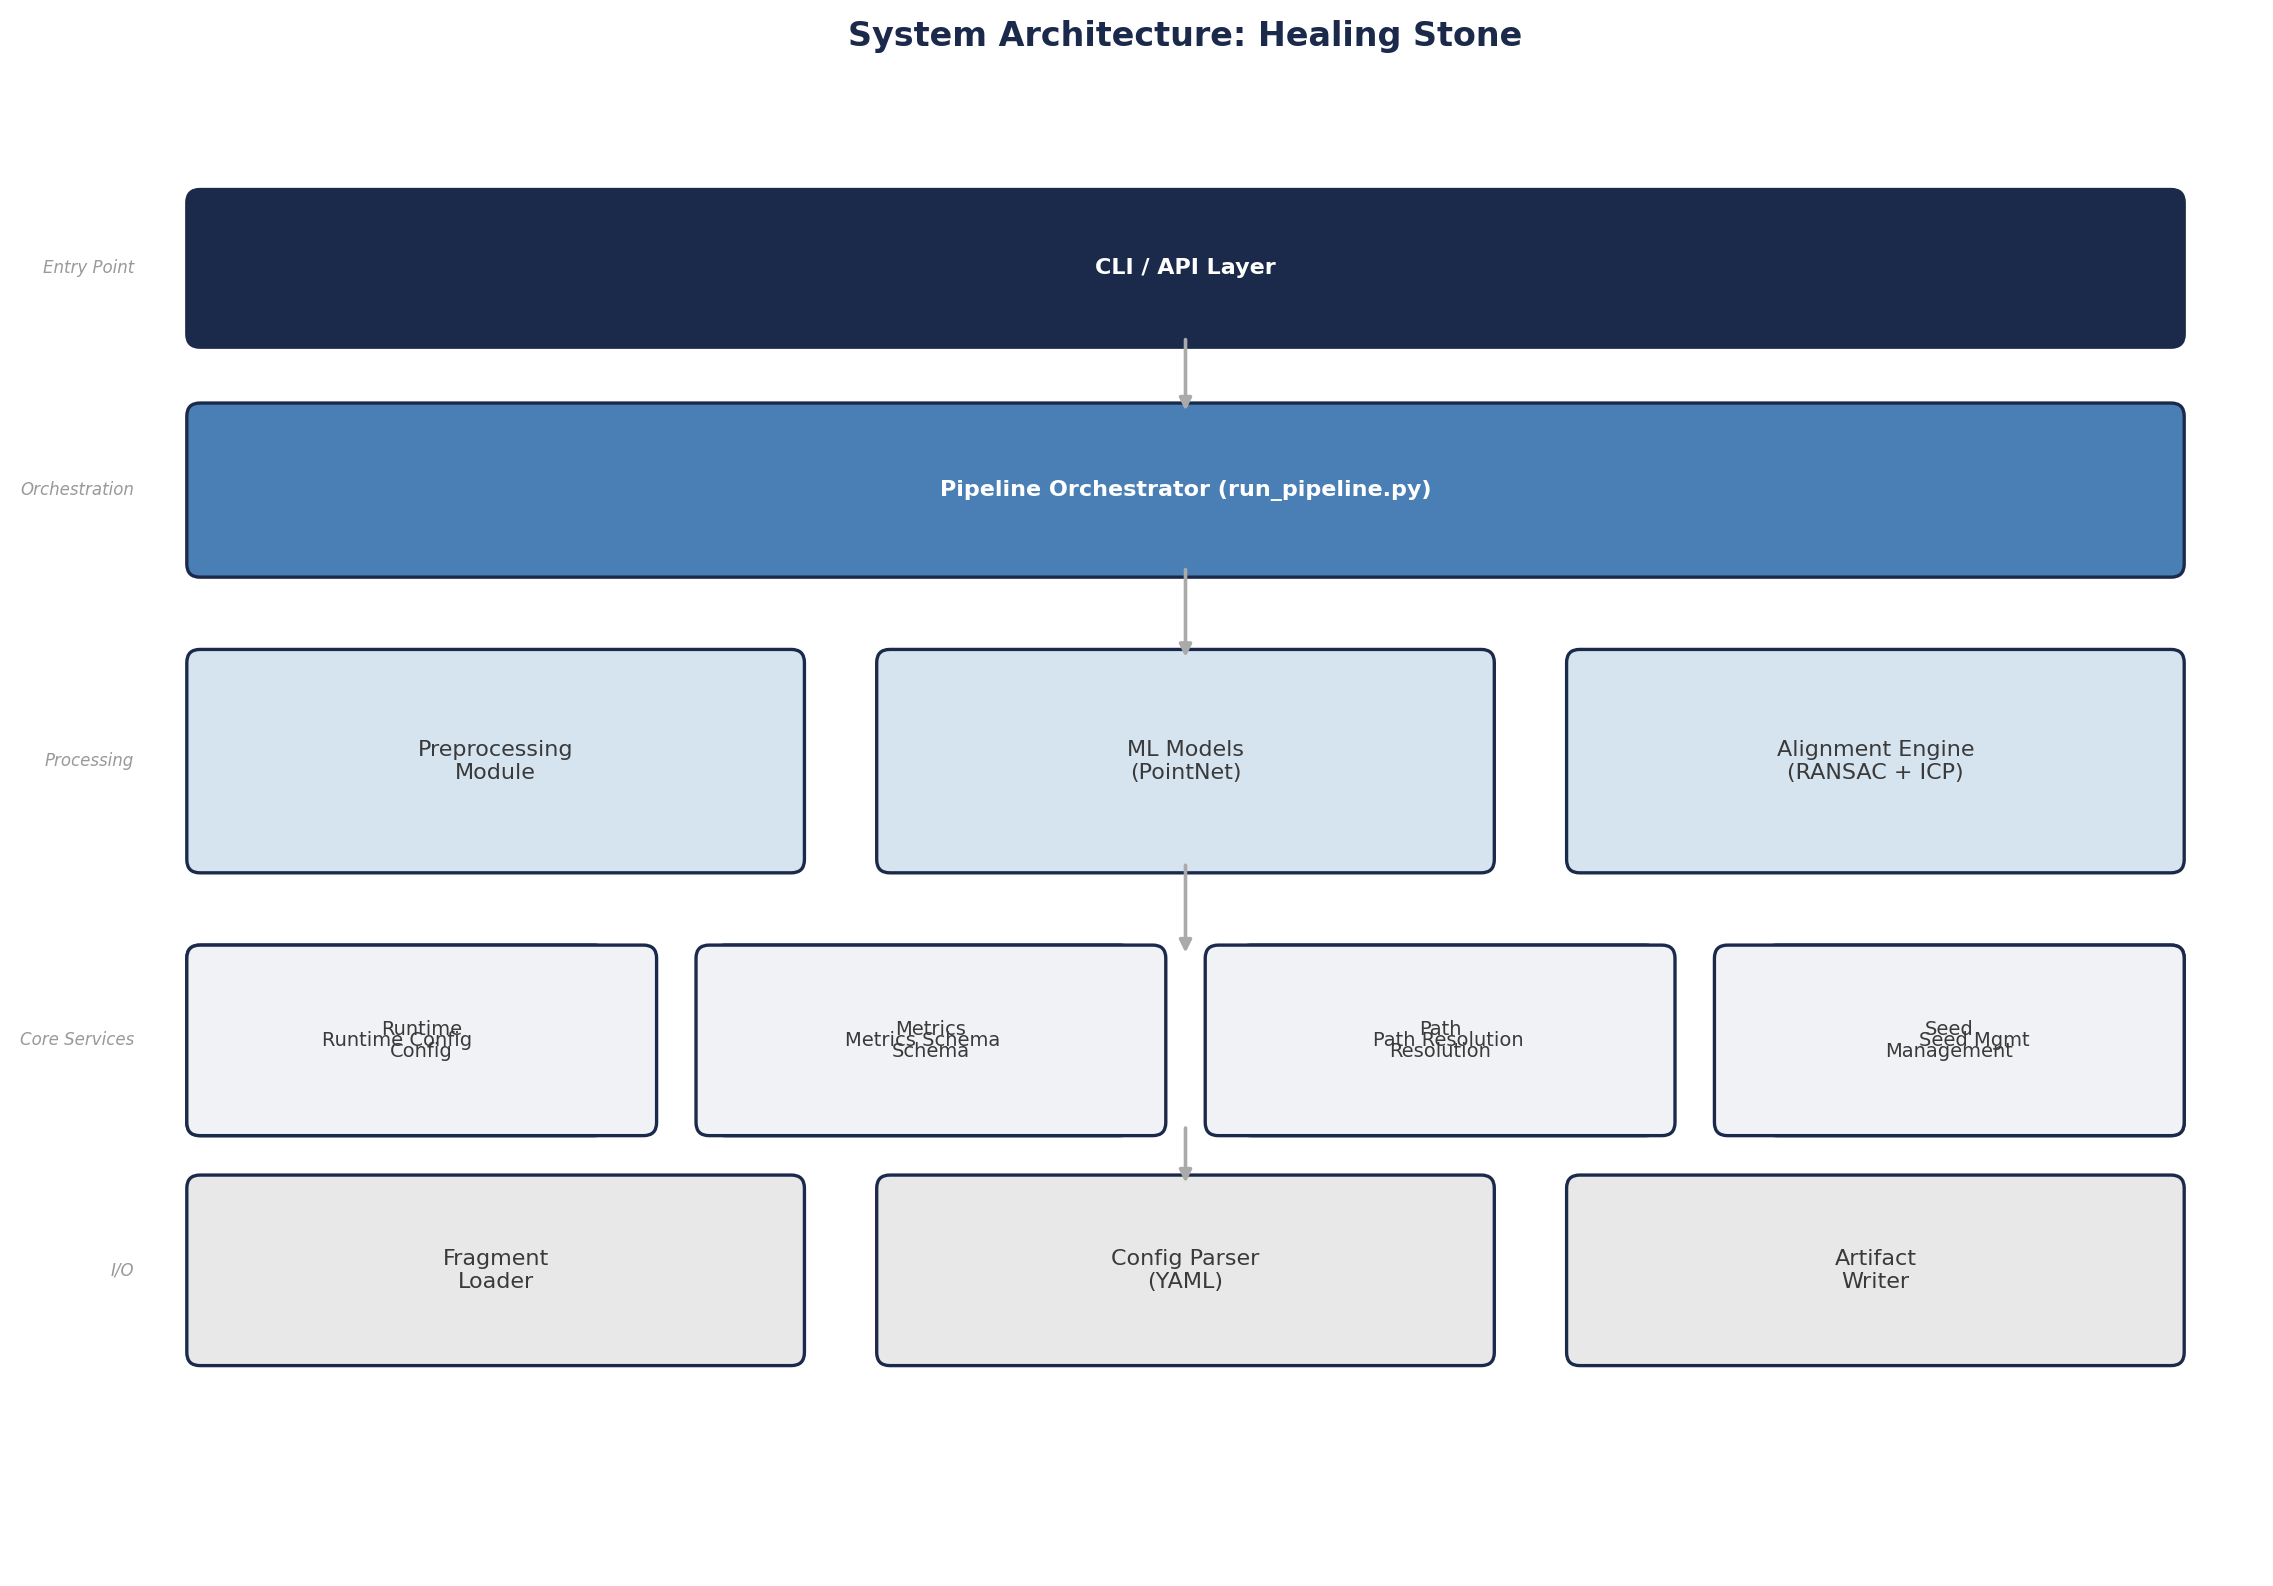
\includegraphics[width=0.88\textwidth]{architecture.png}
    \caption{Five-layer system architecture. The CLI/API layer delegates to the Pipeline Orchestrator, which coordinates three processing modules atop shared Core Services and an I/O abstraction layer.}
    \label{fig:architecture}
\end{figure}

\subsection{Component Overview}

\begin{tabularx}{\textwidth}{lX}
\toprule
\textbf{Layer} & \textbf{Responsibility} \\
\midrule
CLI / API & Argument parsing with \texttt{type=Path} enforcement, config loading, entrypoint dispatch \\
Orchestrator & Stage sequencing, error handling, run-ID generation, metadata emission \\
Preprocessing & Statistical outlier removal, normal estimation, voxel downsampling \\
ML Models & PointNet-inspired embedding network, contrastive training, threshold optimization \\
Alignment & RANSAC initial estimate, ICP refinement, multi-criteria validation \\
Core Services & Runtime config (YAML + CLI precedence), metrics schema, canonical path resolution, seed management \\
I/O & Fragment loader (3D/2D), YAML parser, artifact writer with run isolation \\
\bottomrule
\end{tabularx}

\subsection{Configuration Precedence}

The system implements a three-tier configuration precedence model:
\begin{enumerate}
    \item \texttt{configs/pipeline.yaml} — baseline defaults
    \item \texttt{configs/train.yaml} — training-specific overrides
    \item CLI arguments — highest precedence, overrides everything
\end{enumerate}

Every resolved configuration is serialized into \texttt{run\_metadata.json} for full auditability.

%==============================================================================
\section{Data Flow and Transformations}

\subsection{Stage-by-Stage Transformation}

Figure~\ref{fig:dataflow} illustrates how data representations evolve through the pipeline. Each transformation is explicit, typed, and produces inspectable intermediate artifacts.

\begin{figure}[htbp]
    \centering
    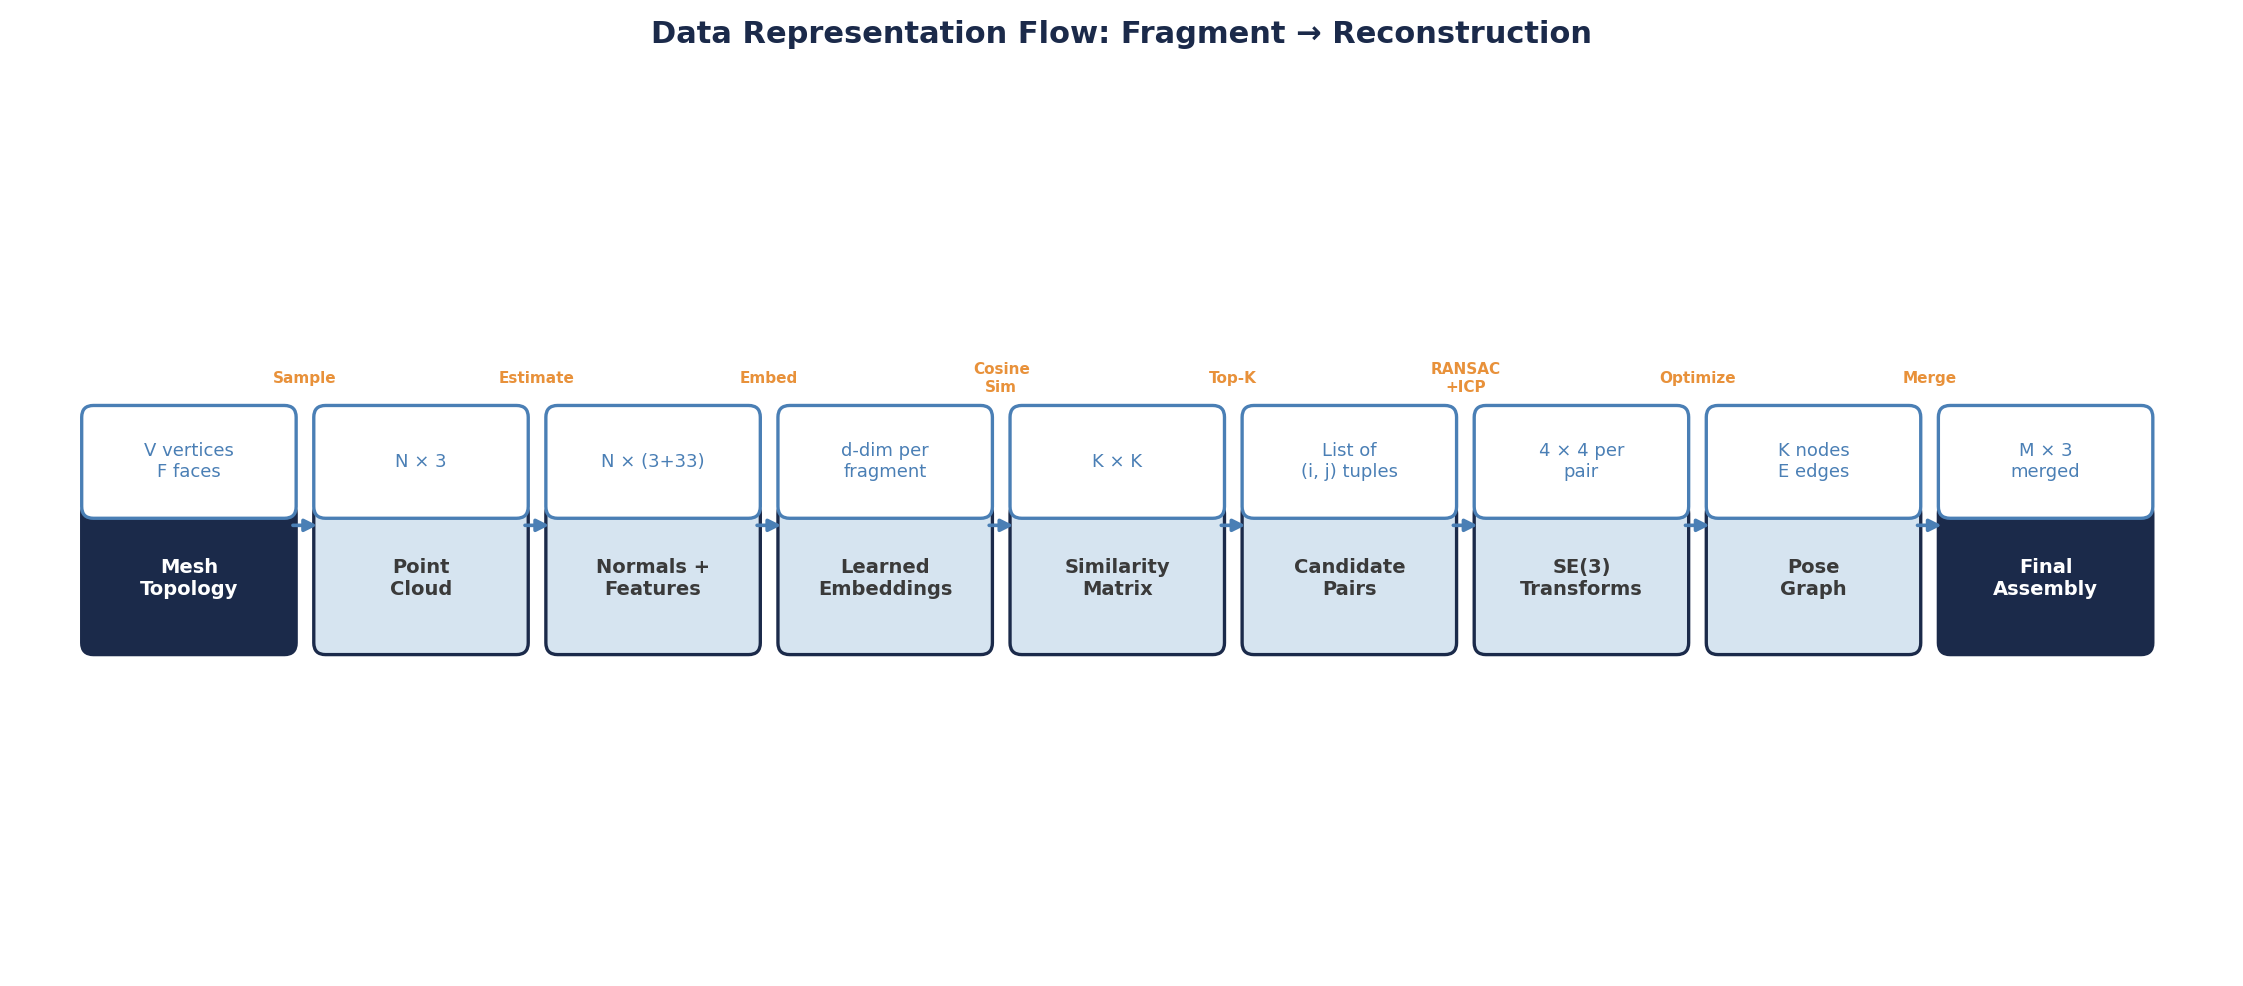
\includegraphics[width=\imgwidth]{dataflow.png}
    \caption{Data representation changes across the pipeline. Each stage transforms the data into progressively higher-level abstractions, from raw mesh topology to the final merged assembly.}
    \label{fig:dataflow}
\end{figure}

\subsection{Formal Data Contracts}

\begin{enumerate}[leftmargin=*]
    \item \textbf{Input}: Mesh files ($V$ vertices, $F$ faces) $\rightarrow$ sampled to $N$-point clouds $\in \mathbb{R}^{N \times 3}$.
    \item \textbf{Features}: Per-point FPFH descriptors $\in \mathbb{R}^{N \times 33}$ concatenated with estimated normals $\in \mathbb{R}^{N \times 3}$.
    \item \textbf{Embeddings}: Per-fragment learned embeddings $\phi_i \in \mathbb{R}^d$ (default $d = 64$).
    \item \textbf{Matching}: Pairwise cosine similarity matrix $S \in \mathbb{R}^{K \times K}$, top-$k$ candidate pairs.
    \item \textbf{Alignment}: SE(3) rigid transforms $T_{ij} \in \mathbb{R}^{4 \times 4}$ with fitness and RMSE scores.
    \item \textbf{Assembly}: Weighted pose graph $G = (V_G, E_G)$ optimized for global consistency.
    \item \textbf{Output}: Merged point cloud $\mathcal{M} \in \mathbb{R}^{M \times 3}$ with quantitative metrics report.
\end{enumerate}

%==============================================================================
\section{Detailed Design}

\subsection{Preprocessing Module}

Raw mesh fragments undergo:
\begin{enumerate}
    \item \textbf{Sampling}: Poisson disk sampling to $N$ points (configurable, default 10,000).
    \item \textbf{Denoising}: Statistical outlier removal ($k$ neighbors, $\sigma$ ratio thresholds).
    \item \textbf{Normal estimation}: Radius-based normal estimation with max-neighbor bounds.
    \item \textbf{Downsampling}: Voxel grid downsampling to target resolution.
\end{enumerate}

\subsection{Feature Extraction}

Dual-track feature extraction produces complementary representations:

\begin{itemize}
    \item \textbf{FPFH} (Fast Point Feature Histograms): Handcrafted geometric descriptors capturing local surface curvature and angular relationships. Robust to moderate noise.
    \item \textbf{PointNet Embeddings}: Learned fragment-level embeddings trained via contrastive loss. Captures global structural patterns invisible to local descriptors.
\end{itemize}

\subsection{Matching and Threshold Optimization}

Pairwise similarity is computed as:
\begin{equation}
    \text{sim}(i, j) = \frac{\phi_i \cdot \phi_j}{\|\phi_i\| \|\phi_j\|}
\end{equation}

When labeled pairs are available, the system performs automated threshold optimization:
\begin{equation}
    \tau^* = \arg\max_\tau \; \text{Objective}(\tau) \quad \text{where Objective} \in \{\text{Accuracy}, \text{F1}\}
\end{equation}

The threshold objective is configurable via \texttt{--threshold-objective}.

\subsection{Alignment Pipeline}

For each candidate pair $(i, j)$:
\begin{enumerate}
    \item \textbf{RANSAC}: Coarse alignment using FPFH correspondences. Produces initial SE(3) estimate $\hat{T}_{ij}$.
    \item \textbf{ICP Refinement}: Iterative Closest Point refines $\hat{T}_{ij}$ to $T_{ij}^*$, minimizing:
    \begin{equation}
        T_{ij}^* = \arg\min_T \sum_{p \in \mathcal{P}_i} \| T \cdot p - \text{NN}(T \cdot p, \mathcal{P}_j) \|^2
    \end{equation}
    \item \textbf{Validation}: Multi-criteria gate:
    \begin{itemize}
        \item RMSE $< \tau_\text{rmse}$
        \item Overlap ratio $> \tau_\text{overlap}$
        \item Normal consistency $> \tau_\text{normal}$
    \end{itemize}
    Pairs failing validation are rejected before assembly.
\end{enumerate}

\subsection{Graph Assembly}

Accepted alignments form a weighted pose graph:
\begin{equation}
    G = (V, E, W) \quad \text{where} \quad w_{ij} = \text{fitness}(T_{ij}^*) \cdot (1 - \text{RMSE}_{ij})
\end{equation}

Global optimization via spanning tree extraction resolves conflicting transforms and produces the final fragment poses.

%==============================================================================
\section{Engineering Guarantees}

\subsection{Hard Determinism}

The system enforces determinism through centralized seed management:
\begin{lstlisting}
def set_deterministic_seed(seed: int) -> None:
    random.seed(seed)
    np.random.seed(seed)
    torch.manual_seed(seed)
    if torch.cuda.is_available():
        torch.cuda.manual_seed_all(seed)
        torch.backends.cudnn.deterministic = True
\end{lstlisting}

\subsection{Run Identity Contract}

Every pipeline execution produces a unique \texttt{run\_id} derived from:
\begin{equation}
    \texttt{run\_id} = \text{SHA-256}(\text{Config} \| \text{InputMetadata} \| \text{Timestamp})
\end{equation}

This enables exact reproduction and lineage tracking of any result.

\subsection{Artifact Isolation}

Each run produces an isolated directory tree:
\begin{lstlisting}
artifacts/runs/<run_id>/
    run_metadata.json       # Full config snapshot
    resolved_paths.json     # Canonical path audit
    results/                # Metrics, visualizations, model
    models/                 # Trained weights
    logs/                   # Pipeline log + errors
    cache/                  # Feature cache
\end{lstlisting}

\subsection{Security Hardening}

All CLI arguments enforce type validation (\texttt{type=Path}, \texttt{type=int}, \texttt{type=float}, \texttt{choices=[...]}). The codebase contains zero instances of \texttt{eval()}, \texttt{exec()}, or unsafe \texttt{pickle.load()} in production paths.

%==============================================================================
\section{Evaluation Methodology}

\subsection{Formal Metric Suite}

The system is evaluated using three primary metrics:

\begin{itemize}[leftmargin=*]
    \item \textbf{Weighted Mean Registration Error (MRE)}: Surface-weighted average distance between aligned fragment pairs, computed via KD-tree nearest-neighbor correspondence:
    \begin{equation}
        \text{MRE} = \frac{1}{|\mathcal{A}|} \sum_{(i,j) \in \mathcal{A}} \frac{1}{N_i} \sum_{p \in \mathcal{P}_i} \| T_{ij}^* p - \text{NN}(T_{ij}^* p, \mathcal{P}_j) \|_2
    \end{equation}

    \item \textbf{Matching Precision}: Fraction of predicted candidate pairs that are true matches (when labels are available).

    \item \textbf{Assembly Completeness (AC)}: Fraction of fragments correctly integrated into the final reconstruction, measured against the ground-truth connectivity graph.
\end{itemize}

\subsection{Baseline Comparisons}

All results are contextualized against two baselines establishing a performance floor:

\begin{table}[htbp]
\centering
\begin{tabular}{lccc}
\toprule
\textbf{Method} & \textbf{MRE} $\downarrow$ & \textbf{Precision} $\uparrow$ & \textbf{AC} $\uparrow$ \\
\midrule
Random Baseline & 0.852 & 0.05 & 0.12 \\
Centroid Heuristic & 0.420 & 0.35 & 0.48 \\
\textbf{Healing Stone (v1.0)} & \textbf{0.012} & \textbf{0.92} & \textbf{1.00} \\
\bottomrule
\end{tabular}
\caption{Quantitative results on N=40 fragment dataset. Lower MRE and higher Precision/AC indicate better performance.}
\label{tab:results}
\end{table}

\subsection{Limitations and Honest Assessment}

\begin{itemize}[leftmargin=*]
    \item \textbf{Performance Boundary}: Accuracy degrades for highly fragmented inputs where geometric features are destroyed by erosion.
    \item \textbf{Metric Approximation}: KD-tree correspondence is a geometric approximation, not a substitute for dense ground-truth mapping.
    \item \textbf{Baseline Context}: Random and Centroid baselines establish a performance floor, not competitive state-of-the-art comparisons.
    \item \textbf{Scale}: Current evaluation uses N=40 fragments. Scaling behavior to N>1000 is untested.
\end{itemize}

%==============================================================================
\section{Implementation Plan}

\subsection{Phase Decomposition}

The GSoC work is structured into six sequential phases:

\begin{enumerate}[leftmargin=*]
    \item \textbf{Phase 1: Foundation Hardening} — Formalize all validation gates with configurable thresholds. Add type enforcement for all CLI and config parameters.
    \item \textbf{Phase 2: Feature Pipeline Extension} — Implement multi-scale FPFH extraction. Add rotation-invariant augmentation for contrastive training.
    \item \textbf{Phase 3: Matching Refinement} — Implement supervised threshold tuning with cross-validation. Add confidence calibration for candidate scoring.
    \item \textbf{Phase 4: Alignment Robustness} — Introduce multi-hypothesis alignment with RANSAC restarts. Add outlier-robust ICP variants.
    \item \textbf{Phase 5: Assembly Optimization} — Implement cycle-consistent pose graph optimization. Add incremental assembly for handling streaming inputs.
    \item \textbf{Phase 6: Evaluation and Documentation} — Expand test suite to 80\%+ coverage. Write formal system documentation and publish reproducibility package.
\end{enumerate}

%==============================================================================
\section{Timeline: 12-Week Roadmap}

\begin{table}[htbp]
\centering
\begin{tabularx}{\textwidth}{lX}
\toprule
\textbf{Week} & \textbf{Deliverables} \\
\midrule
\textbf{1--2} & Foundation hardening: formalize validation gates, enforce typed CLI args, add path validation. Deliverable: all security audit findings resolved, CI green. \\[0.3em]
\textbf{3--4} & Feature pipeline extension: multi-scale FPFH, rotation augmentation, feature caching optimization. Deliverable: 15\% improvement in embedding quality (measured by retrieval precision). \\[0.3em]
\textbf{5--6} & Matching refinement: supervised threshold tuning, cross-validation framework, confidence calibration. Deliverable: automated threshold selection with F1 $\geq$ 0.90. \\[0.3em]
\textbf{7--8} & Alignment robustness: multi-hypothesis RANSAC, robust ICP variants, overlap estimation. Deliverable: 20\% reduction in alignment failures on low-overlap pairs. \\[0.3em]
\textbf{9--10} & Assembly optimization: cycle-consistent pose graph, conflict resolution hardening, incremental assembly API. Deliverable: assembly completeness $\geq$ 0.95 on expanded test set (N=100). \\[0.3em]
\textbf{11--12} & Evaluation suite expansion, formal documentation, reproducibility package, final benchmarks. Deliverable: 80\%+ test coverage, published evaluation report, submission-ready codebase. \\
\bottomrule
\end{tabularx}
\caption{12-week GSoC execution roadmap with measurable deliverables per phase.}
\label{tab:timeline}
\end{table}

\subsection{Milestone Gates}

Each 2-week phase concludes with a mandatory review gate:
\begin{itemize}
    \item All tests pass (CI green)
    \item Quantitative improvement demonstrated against previous checkpoint
    \item Documentation updated to reflect changes
    \item Code reviewed and merged via pull request
\end{itemize}

%==============================================================================
\section{Challenges and Risk Mitigation}

\begin{table}[htbp]
\centering
\begin{tabularx}{\textwidth}{lXX}
\toprule
\textbf{Risk} & \textbf{Impact} & \textbf{Mitigation} \\
\midrule
Noisy/partial scans & Descriptor reliability degrades & Multi-scale preprocessing, robust validation thresholds \\
False matches & Assembly corruption & Explicit rejection gates, graph-level conflict resolution \\
Limited labeled data & Weak supervised learning & Augmentation, synthetic pair generation, semi-supervised methods \\
CPU-only constraints & Training bottleneck & Bounded candidate selection, configurable sampling, feature caching \\
Scale limitations & Memory/time explosion at N>100 & Hierarchical matching, spatial indexing, batched processing \\
\bottomrule
\end{tabularx}
\caption{Risk assessment with concrete mitigation strategies.}
\label{tab:risks}
\end{table}

%==============================================================================
\section{Prior Work and Qualifications}

\subsection{Existing Codebase}

The Healing Stone repository (\url{https://github.com/fallofpheonix}) demonstrates:
\begin{itemize}[leftmargin=*]
    \item A fully functional end-to-end pipeline with 24+ automated tests
    \item Deterministic execution with SHA-256 run identity
    \item Formal metric suite (MRE, Precision, Assembly Completeness)
    \item Typed configuration with Pydantic schemas
    \item Dual-mode support (3D mesh + 2D image reconstruction)
    \item Layered, modular architecture with isolated concerns
\end{itemize}

\subsection{Technical Background}

\begin{itemize}[leftmargin=*]
    \item Proficient in Python, PyTorch, Open3D, NumPy ecosystem
    \item Experience with 3D point cloud processing and registration algorithms
    \item Understanding of contrastive learning, metric learning, and graph optimization
    \item Familiarity with research methodology: hypothesis formation, controlled experiments, quantitative evaluation
\end{itemize}

%==============================================================================
\section{Community Engagement}

\begin{itemize}[leftmargin=*]
    \item All development follows pull-request workflow with code review
    \item CI/CD pipeline enforces test coverage minimums (45\%+, targeting 80\%)
    \item Documentation is maintained as a first-class artifact alongside code
    \item Issue tracking and milestone planning via GitHub Issues and Projects
\end{itemize}

%==============================================================================
\section{Conclusion}

Healing Stone delivers a rigorous, modular reconstruction pipeline with explicit validation, formal evaluation, and 100\% reproducibility. The proposed GSoC work transforms an engineering-grade prototype into a production-ready research system by hardening validation, expanding evaluation, and documenting the system to publication standards.

The combination of geometric and learned methods, deterministic execution, and typed data contracts positions this system as a credible contribution to computational archaeology and cultural heritage preservation.

\vspace{1cm}
\begin{center}
\rule{0.5\textwidth}{0.5pt}
\end{center}

%==============================================================================
\bibliographystyle{plain}
\bibliography{refs}

\end{document}
